\documentclass{article}
\usepackage[utf8]{inputenc}

\title{COMP 138 RL: Assignment 1}
\author{Luxi Liu}

\usepackage{natbib}
\usepackage{graphicx}

\begin{document}

\maketitle

\section{Introduction}
The k-armed Bandit Problem is a nonassociative problem where, faced with k choices, we seek to optimize the total reward over some period. 

We can estimate the reward for a certain arm based on the average of the rewards we have received so far, i.e. the Sample Average method: $$Q_{n+1} = Q_n + \frac{1}{n} (R_n - Q_n)$$

Alternativley, we can calculate the estimated reward by giving more weight to recent rewards, using a constant step-size parameter $\alpha$, this is called the Exponential Recency-Weighted Average method: $$Q_{n+1} = Q_n + \alpha (R_n - Q_n)$$

\section{Problem Statement}
We want to design and conduct an experiment to demonstrate the
difficulties that sample-average methods have for nonstationary problems. 

For this purpose, we use a 10-armed testbed. The rewards of each arm start off as a normal distribution with mean 0, deviation 1, we run the experiment for 1000 times, each time we run 10,000 steps (to keep things consistent, the above parameters will not change through the rest of the experiments). Each arm takes independent random walk by adding a normally distributed increment with mean 0 and standard deviation 0.01. 

We compare the results, average rewards and the proportion that the optimal action is selected, using the Sample Average method versus using the Exponential Recency-Weighted Average method.

\section{Experiment}
\subsection{Basic Hypothesis}
Overall, I hypothesize that the Sample Average will do worse than the Exponential Recency-Weighted Average method since it does not give more weights to more recent changes. In a nonstationary problem, recent changes should have more effects on overall rewards. I also guess that this will be more obvious in the long run since the distribution of rewards have moved further away from initial values.

\begin{figure}[h!]
\centering
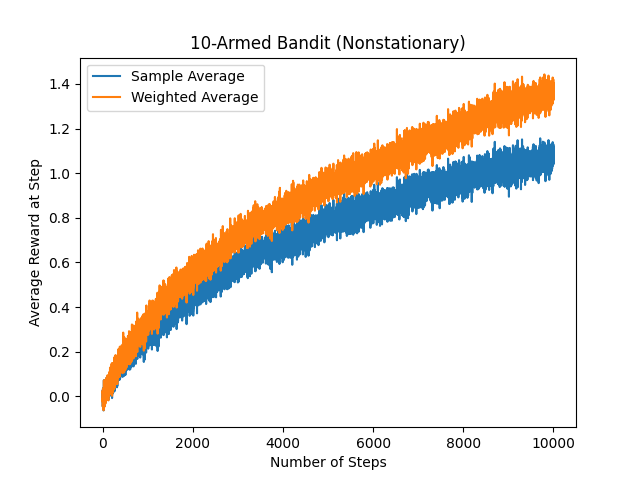
\includegraphics[scale=.6]{RL_A1_pics/dif_arms/num_steps=10000, num_experiments=1000, arms=10, var=1, rand_walk_var=0.01, alpha=0.1, epsilon=0.1.png}
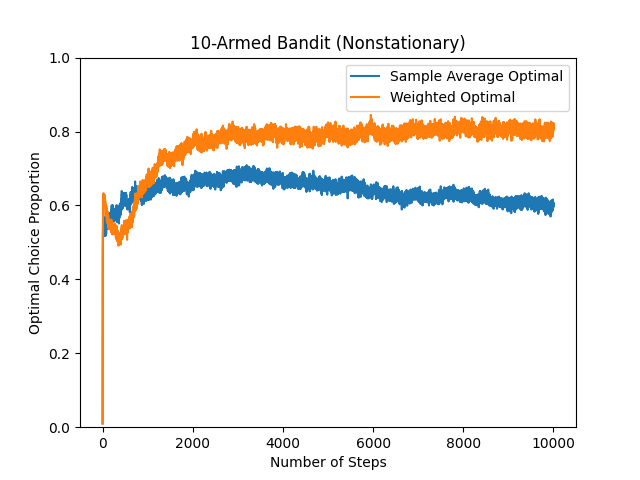
\includegraphics[scale=.6]{RL_A1_pics/dif_arms/optimal/10.png}
\caption{random walk variance = 0.01, $\epsilon$ = 0.1, $\alpha$ = 0.1}
\label{fig:10-Armed1}
\end{figure}

The result graph confirms our assumption that Sample Average does worse than Exponential Recency-Weighted Average in nonstationary problem, and the proportion of selecting optimal choice goes down as number of steps grows.

For comparison, we set up a stationary problem, the 10 arms each has a random mean from a normal distribution of mean 0, variance 1, we can see that the Sample Average method performs significantly better than in the nonstationary problem, it also performs better than the weighted method (as it would not help in stationary problems to give more weights on more recent changes), showing that Sample Average is a good method for stationary problems:

\begin{figure}[h!]
\centering
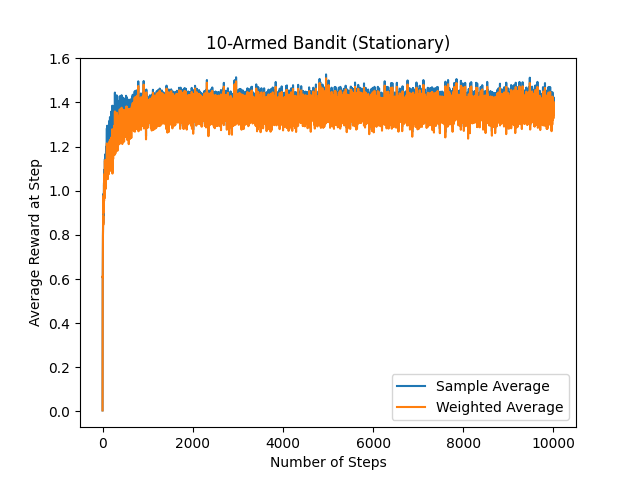
\includegraphics[scale=.6]{RL_A1_pics/mean0var1randomMeans.png}
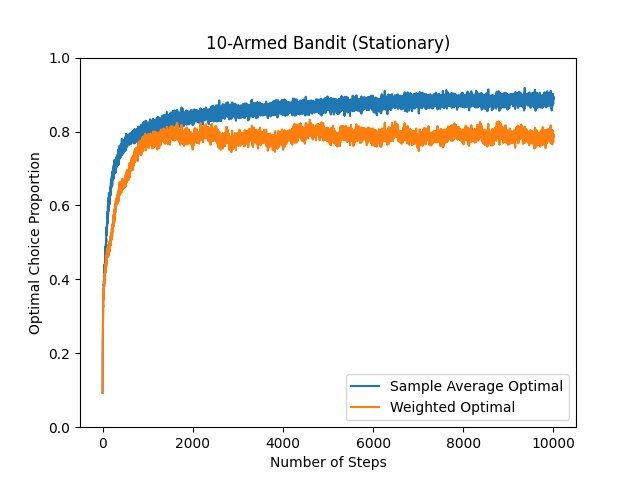
\includegraphics[scale=.6]{RL_A1_pics/mean0var1randomMeans_optimal.png}
\caption{\textbf{random walk variance = 0}, $\epsilon$ = 0.1, $\alpha$ = 0.1}
\label{fig:10-Armed1}
\end{figure}


\subsection{Difference in Random Walk Variance}
Then, I hypothesize that the steeper the change (e.g. set the variance for random walk to be higher), the worse that Sample Average method will do.

\begin{figure}[h!]
\centering
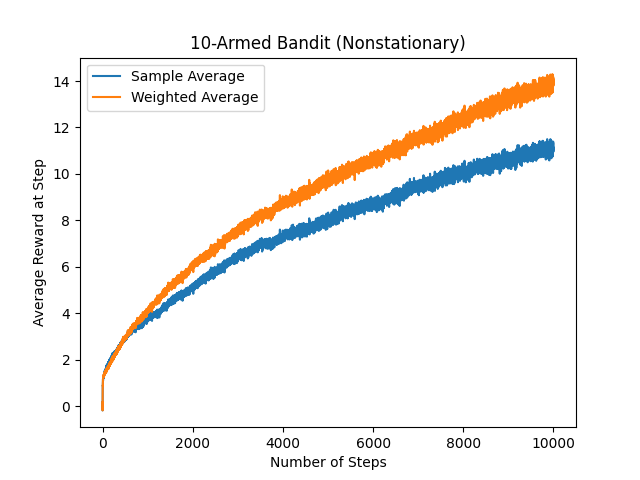
\includegraphics[scale=.6]{RL_A1_pics/rand_walk_var/0.1.png}
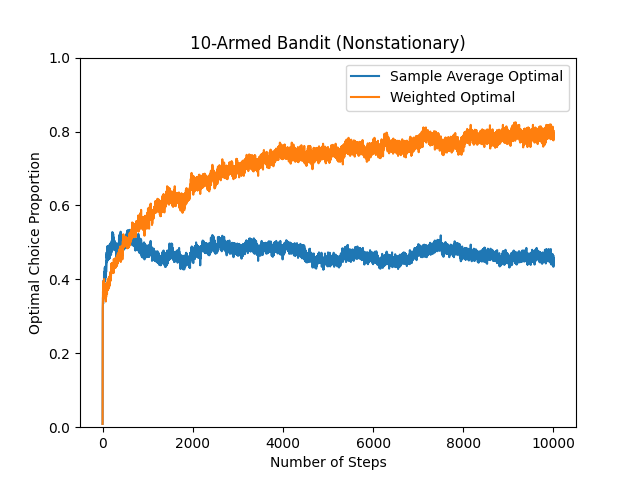
\includegraphics[scale=.6]{RL_A1_pics/rand_walk_var/optimal/0.1.png}
\caption{\textbf{random walk variance = 0.1}, $\epsilon$ = 0.1, $\alpha$ = 0.1}
\label{fig:10-Armed1}
\end{figure}

\begin{figure}[h!]
\centering
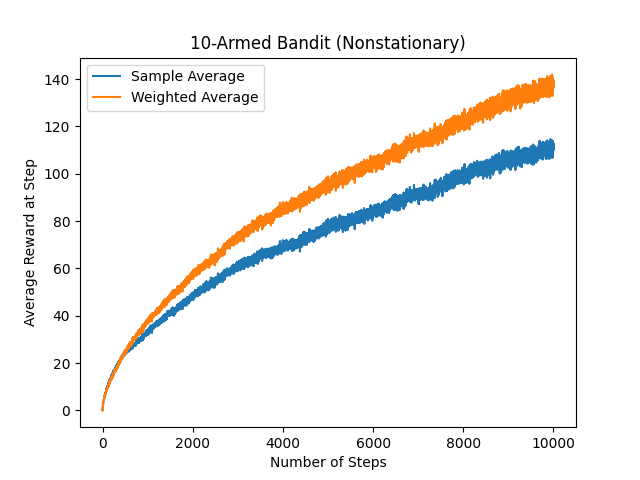
\includegraphics[scale=.6]{RL_A1_pics/rand_walk_var/1.png}
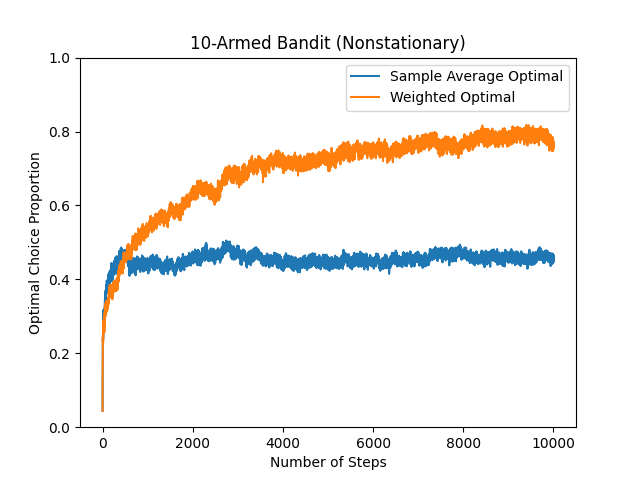
\includegraphics[scale=.6]{RL_A1_pics/rand_walk_var/optimal/1.png}
\caption{\textbf{random walk variance = 1}, $\epsilon$ = 0.1, $\alpha$ = 0.1}
\label{fig:10-Armed1}
\end{figure}

\newpage
This result also confirms our assumption: the proportion for optimal result for the weighted method stabilized around 0.8 for random walk variance = 0.01, 0.1, 1, whereas the proportion for Sample Average method went from around 0.6 to 0.5 to lower, although the change from 0.1 to 1 brought less of a change in performance compared to the 0.01 to 0.1 change.

\subsection{Difference in Epsilon}
Next, we try to see if changing the $\epsilon$ could improve the performance for both methods. I would guess increase $\epsilon$ to a certain value could help in nonstationary problem as it increases sensitivity to change, but if we increase $\epsilon$ too much the algorithm becomes more random thus impair performance.

\begin{figure}[h!]
\centering
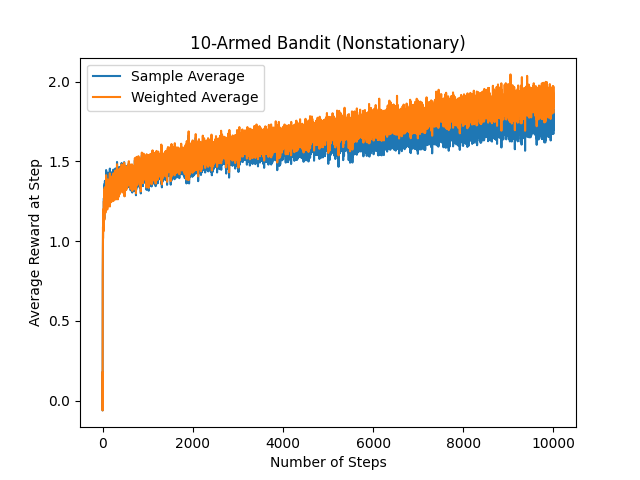
\includegraphics[scale=.6]{RL_A1_pics/epsilon/0.2.png}
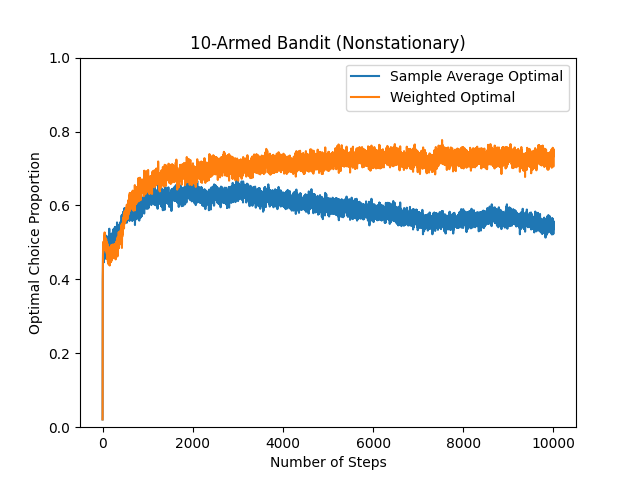
\includegraphics[scale=.6]{RL_A1_pics/epsilon/optimal/0.2.png}
\caption{random walk variance = 0.01, \textbf{$\epsilon$ = 0.2}, $\alpha$ = 0.1}
\label{fig:10-Armed1}
\end{figure}

\begin{figure}[h!]
\centering
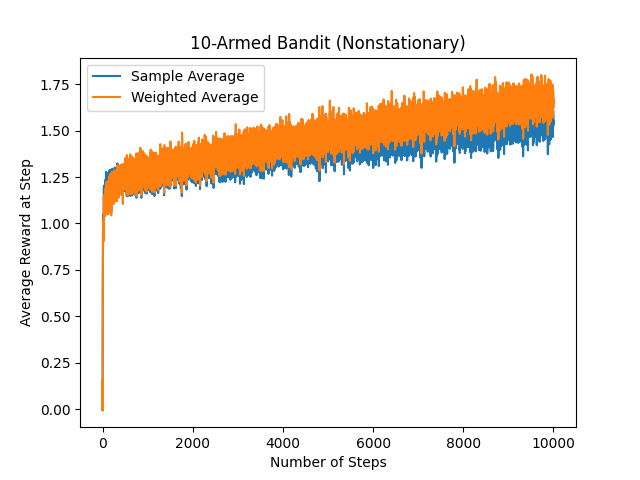
\includegraphics[scale=.6]{RL_A1_pics/epsilon/0.3.png}
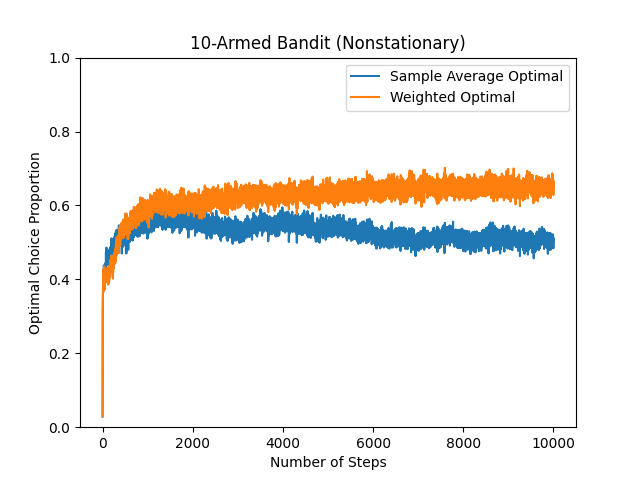
\includegraphics[scale=.6]{RL_A1_pics/epsilon/optimal/0.3.png}
\caption{random walk variance = 0.01, \textbf{$\epsilon$ = 0.3}, $\alpha$ = 0.1}
\label{fig:10-Armed1}
\end{figure}

\newpage
We see that increasing $\epsilon$ actually does not help the performance in either of the methods, compared to our original $\epsilon = 0.1$. It could be due to that the distribution is not changing fast enough to be requiring a larger $\epsilon$, therefore, the increase in randomness just decreased our overall reward. In addition, decreasing $\epsilon$ to 0.01 seems to have a slight positive effect on performance:

\begin{figure}[h!]
\centering
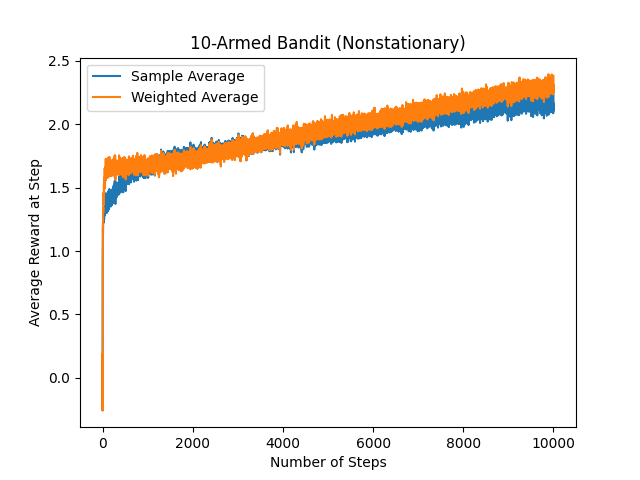
\includegraphics[scale=.6]{RL_A1_pics/epsilon/0.01.png}
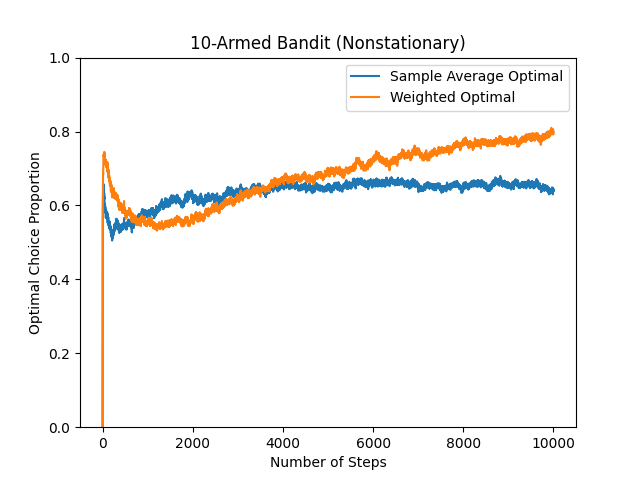
\includegraphics[scale=.6]{RL_A1_pics/epsilon/optimal/0.01.png}
\caption{random walk variance = 0.01, \textbf{$\epsilon$ = 0.01}, $\alpha$ = 0.1}
\label{fig:10-Armed1}
\end{figure}


\subsection{Difference in Alpha}
Next, we are curious about whether changing the $\alpha$ (step-size parameter) will help the performance for the Exponential Recency-Weighted Average method, in this nonstationary problem. Originally (as shown Figure 1), we set random walk variance to 0.01, $\alpha$ to 0.1, so there was a 10 1 to 10 ratio between the two values. 

\begin{figure}[h!]
\centering
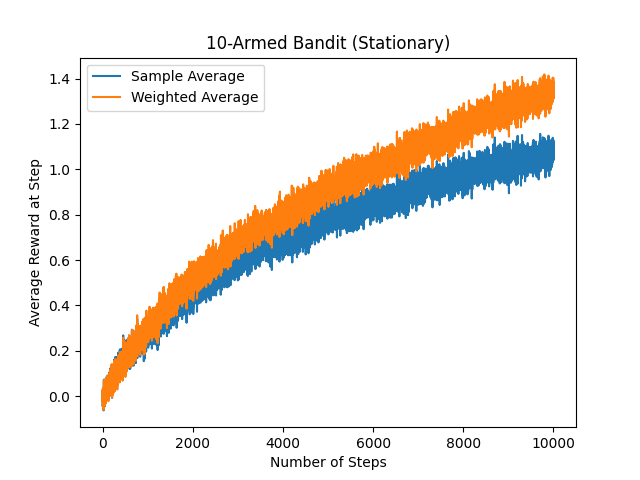
\includegraphics[scale=.6]{RL_A1_pics/alpha/0.2.png}
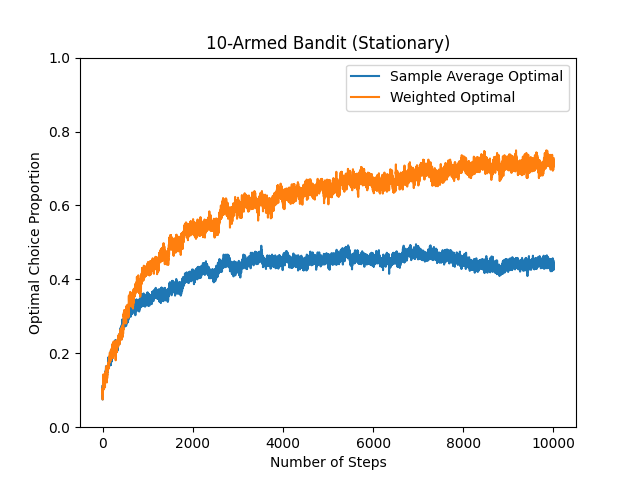
\includegraphics[scale=.6]{RL_A1_pics/alpha/optimal/0.2.png}
\caption{random walk variance = 0.01, $\epsilon$ = 0.1, \textbf{$\alpha$ = 0.2}}
\label{fig:10-Armed1}
\end{figure}

\begin{figure}[h!]
\centering
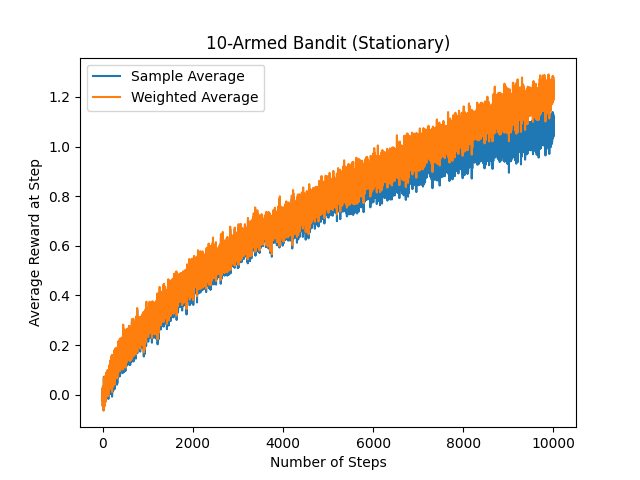
\includegraphics[scale=.6]{RL_A1_pics/alpha/0.01.png}
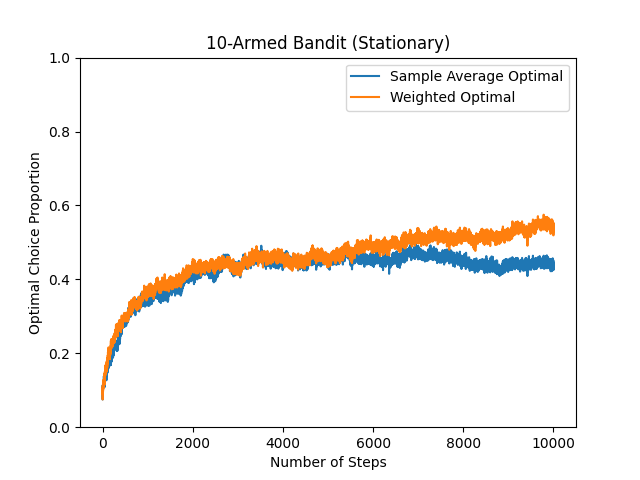
\includegraphics[scale=.6]{RL_A1_pics/alpha/optimal/0.01.png}
\caption{random walk variance = 0.01, $\epsilon$ = 0.1, \textbf{$\alpha$ = 0.01}}
\label{fig:10-Armed1}
\end{figure}

\newpage
We do not see an increase from setting $\alpha$ to an higher number, it looks like 1 to 10 might be a good ratio between the random walk variance and $\alpha$. To confirm this, we try another experiment that has the same issue where random walk variance = 1 and $\alpha$ = 0.9 (since we don't want to entirely discount previous rewards

\newpage
Nor did we see a performance increase by decreasing $\alpha$. It seems like $\alpha$ = 0.1 is a good value for the 10-armed nonstationary problem. Is this still true with a much larger random walk variance? We test this by setting random walk variance to 1:

\begin{figure}[h!]
\centering
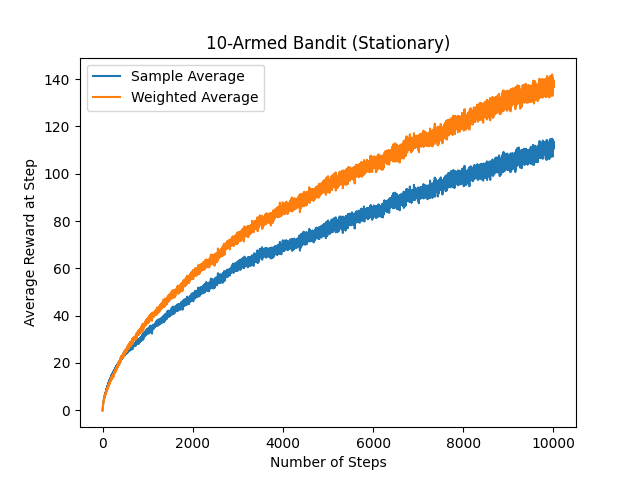
\includegraphics[scale=.6]{RL_A1_pics/alpha/walk1alpha0.1.png}
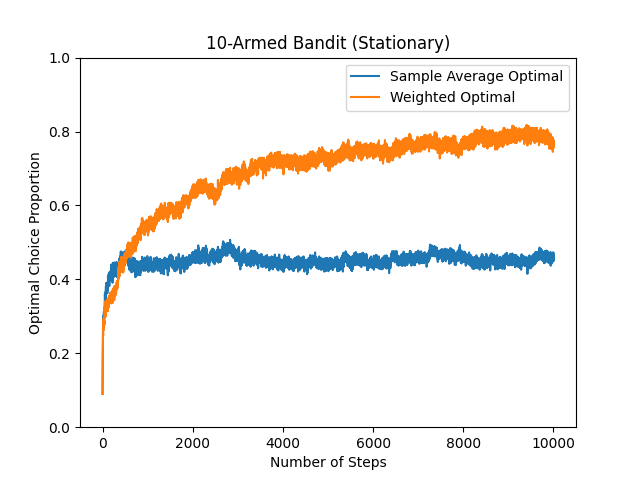
\includegraphics[scale=.6]{RL_A1_pics/alpha/optimal/walk1alpha0.1.png}
\caption{\textbf{random walk variance = 1}, $\epsilon$ = 0.1, \textbf{$\alpha$ = 0.1}}
\label{fig:10-Armed1}
\end{figure}

\newpage
Indeed it turns out $\alpha$ = 0.1 still have very good performance even if random walk variance has increased to 100 times. Although this time, setting $\alpha$ to be 0.2 has a slight boost for performance, which I hypothesize is because the larger random walk variance allows for a bigger $\alpha$, to capture the importance of more recent changes:

\begin{figure}[h!]
\centering
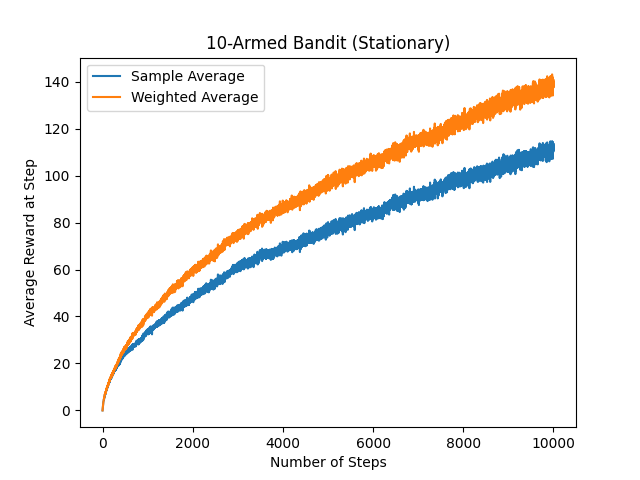
\includegraphics[scale=.6]{RL_A1_pics/alpha/walk1alpha0.2.png}
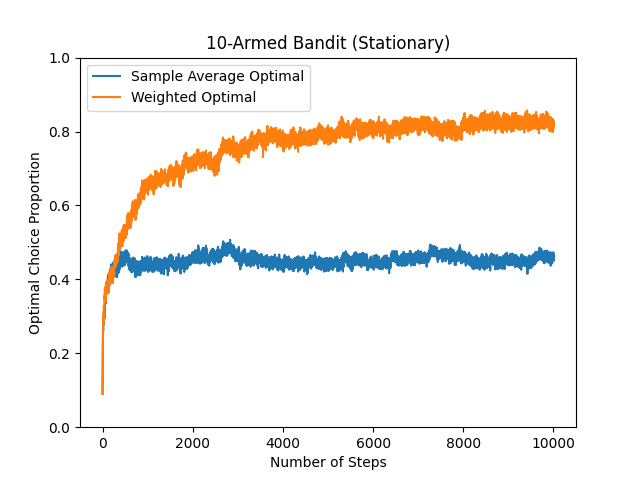
\includegraphics[scale=.6]{RL_A1_pics/alpha/optimal/walk1alpha0.2.png}
\caption{\textbf{random walk variance = 1}, $\epsilon$ = 0.1, \textbf{$\alpha$ = 0.2}}
\label{fig:10-Armed1}
\end{figure}


\subsection{Sudden Change}
Lastly, 


\newpage
\section{Conclusion}
Our experiments shows that Sample Average method does not perform well in nonstationary bandit problems, in comparison, the Exponential Recency-Weighted Average method can stably have much better performance since it decays the rewards that are further back in time. Some possible future research on this problem would be to find the ratio between the amplitude of changes (random walk variance) and the step-size parameter $\alpha$ to optimize performance.

\section{Reference}
The experiments and graph drawing referenced the Sutton and Barto Reinforcement Learning: An Introduction textbook.

\bibliographystyle{plain}
\bibliography{references}
\end{document}
